\documentclass[12pt]{article}
\usepackage{amsmath}
\usepackage{amssymb}
\usepackage{latexsym}
\usepackage{graphicx}
\usepackage{mathrsfs}
\usepackage{CJKutf8}
\author{qit}
\title{暑期培训——进程间的通信}
\begin{document}
\begin{CJK}{UTF8}{gbsn}
\maketitle

\section{进程\&线程的基本概念(看线程)}
\subsection{进程}
\paragraph{}进程可以理解成在os上执行的一个程序的实例。
\paragraph{}比如,我们在PC上开启一个浏览器、word这都是开启了一个个进程。
\subsection{线程}
\paragraph{}线程可以理解为我们一个任务中的子任务,也即一个进程中的多个“子进程”。
\paragraph{}比如,我们在开启word的时候,他可以同时进行打字、自动排版、拼音检查、字数统计等多个任务。即一个word进程下的4个子线程。
\subsection{CPU}
\paragraph{}CPU的一个核心上只能在一个时间片上执行一个进程中的一个线程。对于一个单核心CPU的PC,他仍能同时开启多个进程,每个进程下有多个线程,实现的方法就是由操作系统os进行控制调度,让各个线程在CPU上轮流进行执行,每个线程执行的时间很短,让人感觉上所有任务在同时进行。
\paragraph{}对于n个核心的CPU,他就能够在硬件上真的做到n个线程并行执行。
\paragraph{}但是需要注意的是,对于这种调用是要占用一些时间的,对于计算密集型(时间消耗花费在CPU上)的任务,频繁的切换线程是一件很不划算的事情,CPU的速度是非常快的。对于IO密集型(时间消费花费在和硬盘的IO)的任务,切换线程得到的收益一般会高于不切换线程造成的IO等待。
\subsection{并行\&并发}
\paragraph{并行}多个线程/进程在时间上同步执行。如我们有4个进程,每个进程执行10s,那么并行执行这4个进程,则4个进程在4s后同时执行完。
\paragraph{并发}多个线程/进程交替执行。如我们一个单核CPU,并发执行4个进程,每个进程执行10s,那么4个进程在大于40s后执行完(由于进程的切换)。
\subsection{程序在CPU中的执行方式}
\paragraph{}以C语言为例,首先我们的C语言的代码,会被编译器编译成一条条的汇编指令,汇编指令直接是对CPU中各个寄存器和Memory进行的操作。汇编指令被汇编器专程一条条由01组成的机器码,被我们的CPU识别并执行。
\paragraph{}当我们执行一个程序的时候,首先这个程序对应的机器码会被载入到内存中(简单的情况,不考虑如虚拟内存等技术),之后CPU一条一条的执行这些机器码,即是在执行这个程序。
\paragraph{需要注意的是} 我们的在C语言中的一条命令,如Mem[i+1]=Mem[i]+2对应的汇编语言,可能并不只1条。对于MIPS,会对应5条汇编。但是os在进行线程/进程间的切换的时候,是在执行一定数目的机器码之后进行的切换。因此有可能会出现我们的某一条指令在执行了一半之后os就把我们的这个线程挂起并执行其他线程去了,在涉及到相同内存的IO的时候,会造成一些诡异的问题,需要我们设计来避免这种情况的出现。(进程间通信)\\
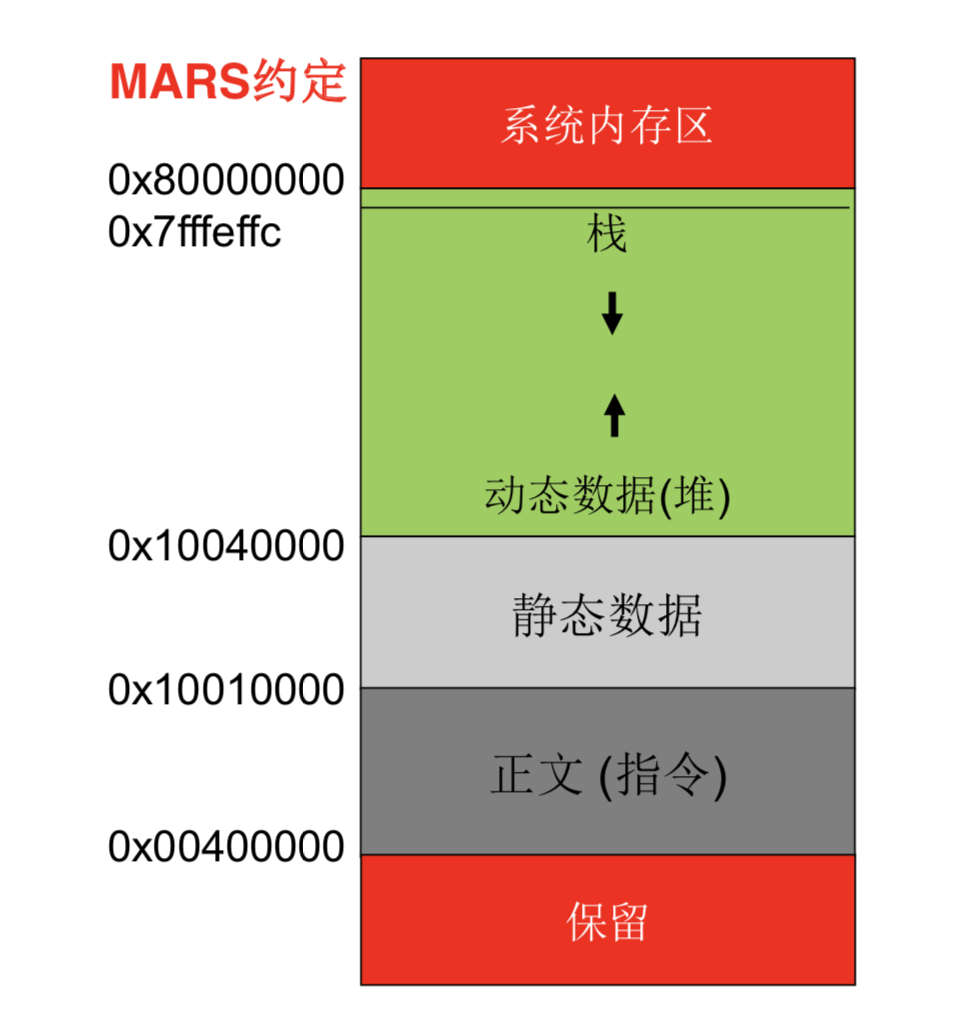
\includegraphics[width=3in]{CPU.png}

\section{多进程}
\subsection{多进程 调用函数}
\subsubsection{多进程编程}
\paragraph{}按照我们之前的理解,一个进程就是一个任务。而我们的一个任务,一般是以一个函数的形式出现(内部的一个任务),或者是可以通过调用一个bash命令来实现(一个外部的任务)。
\subsubsection{内部任务}
\paragraph{1.}from multiprocessing import Process
\\ import os
\paragraph{2.}p=Process(target=target\_func,args=traget\_func\_args)
\\实例化了一个进程类,这个进程会去执行target\_func这个函数,同时target\_func\_args是作为参数传递给这个函数的。
\paragraph{3.}p.start() 启动这个进程
\paragraph{4.}p.join()等待这个进程的结束,没结束就一直阻塞。
\paragraph{5.}os.pid()返回调用这个命令的线程的pid。
\subsubsection{多个内部任务}
\paragraph{1.}from multiprocessing import Pool
\paragraph{2.}p=Pool(n)
\\创建了一个容纳n个进程的进程池。
\paragraph{3.}p.apply\_async(targtet=target\_func\_i,args=arg\_i)
\\把第i个要执行的目标函数和他的参数放入p中,并开始执行。
\\放入的进程数目可以超过n,超过n之后,后放入的目标函数会先等待之前先放入的目标函数执行完之后,才会继续执行。即n代表了最多有开启n个进程同时执行。
\paragraph{4.}p.close()
\\不能继续再向p中放入进程了
\paragraph{5.}p.join()
\\等待所有进程执行完毕
\\在执行p.join()前必须先执行p.close()
\subsubsection{外部任务}
\paragraph{1.}import subprocess
\paragraph{2.}subprocess.call(bash)
\\会执行相应的bash命令。
\paragraph{3.}在写脚本的时候,十分有用。在需要的时候自学其他API。

\section{多线程}
\subsection{python下多线程}
\paragraph{1.}import subprocess
\paragraph{2.}t=threading.Thread(target=target\_fun,args=target\_args)
\\创建一个线程实例
\\执行target\_function,并且把target\_args传递给这个function。
\paragraph{3.}t.start()
\\开始执行
\paragraph{4.}t.join()
\\阻塞,等到t执行完毕。

\subsection{C++下多线程}
\paragraph{}与平台相关,linux下使用pthread库,自学相应API。
\subsection{GIL锁}
\paragraph{}Python的解释器执行代码时,有一个GIL锁:Global Interpreter Lock,任何Python线程执行前,必须先获得GIL锁,然后,每执行100条字节码,解释器就自动释放GIL锁,让别的线程有机会执行。这个GIL全局锁实际上把所有线程的执行代码都给上了锁,所以,多线程在Python中只能交替执行,即使100个线程跑在100核CPU上,也只能用到1个核。因此使用官方python解释器的多线程无法并行执行。


\section{进程/线程间通信}
\subsection{producer-consumer}
\paragraph{}无论是多进程还是多线程,如果他们试图读写同一块内存,那么他们就会出现数据竞争(data race)。需要进行进程间的通信,防止data race的发生。
\paragraph{}将即将读写共享内存的线程称为即将进入临界区的线程。
\paragraph{}之后以producer-consumer模型来分析data race的问题。
\subsubsection{producer-consumer}
\paragraph{producer}向一块size为N的buffer中写入数据,每次写的数据的size为1,buffer满后将无法写入。
\paragraph{consumer}从一块size为N的buffer中读取数据,每次读的数据的size为1,buffer空后将无法读取。


\subsection{忙等待(禁止使用)(例子)}
\paragraph{}忙等待指的是这样一种实现,当一个线程进入临界区之前,需要先判断他能否进入临界区,采用一个循环来不停的判断,直到其他线程退出临界区,条件改变,就能退出循环,这个线程可以进入临界区。
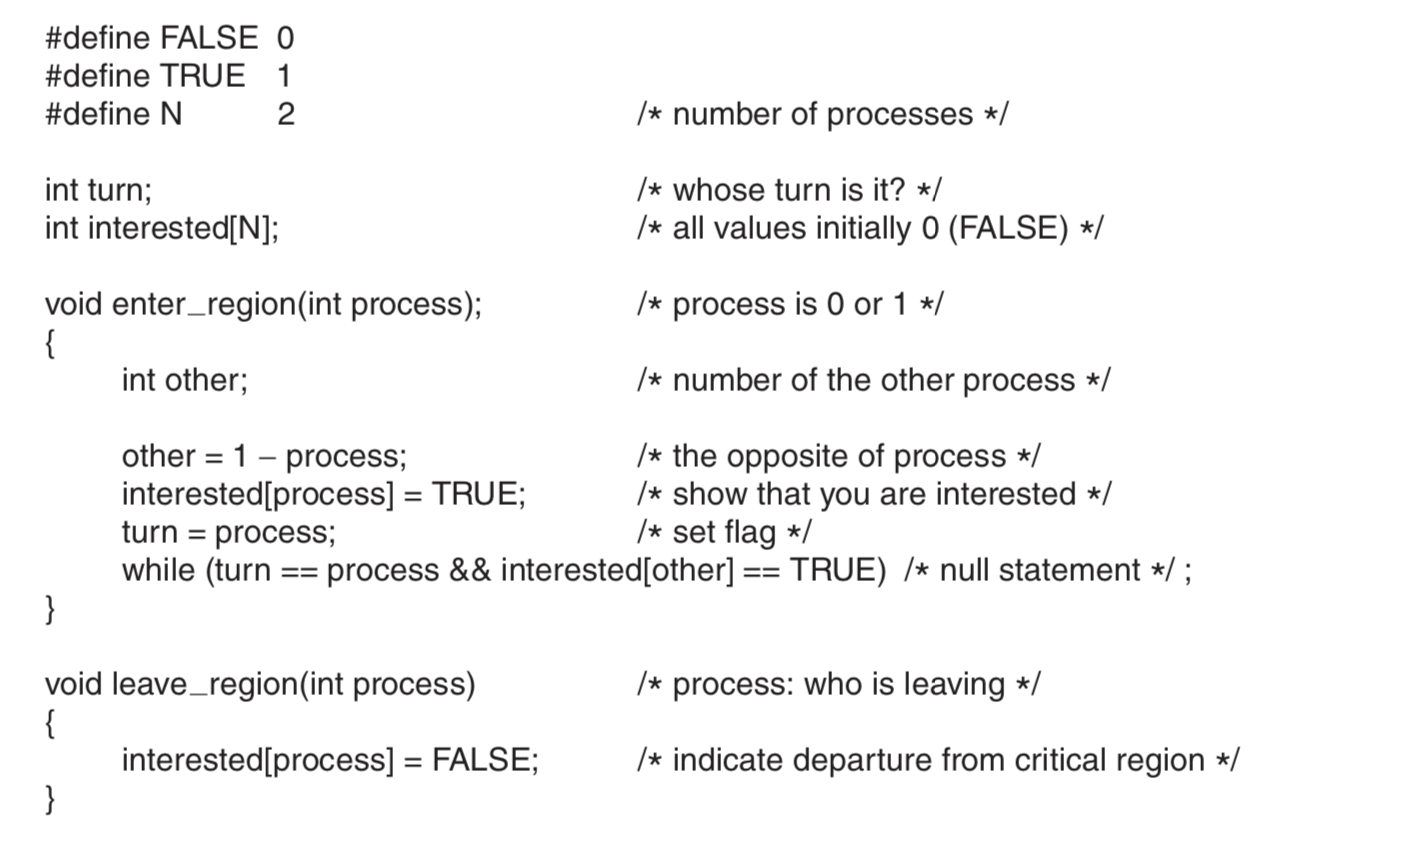
\includegraphics[width=6in]{wait.png}
\paragraph{问题:}忙等待非常的占用CPU时间,正在忙等待的程序会让CPU负荷达到100\%,会对运行在该CPU上的其他线程造成不好的影响。
\subsection{sleep and wakeup(禁止使用)}
\paragraph{}相比于忙等待在无法进入进入临界区时,不断通过循环来判断,sleep和wakeup是使线程在无法进入临界区的时候sleep,并且在能够进入临界区的时候被其他线程唤醒。
\paragraph{}相比于忙等待的优点,就在于忙等待非常的占用CPU时间,正在忙等待的程序会让CPU负荷达到100\%,会对运行在该CPU上的其他线程造成不好的影响。\\
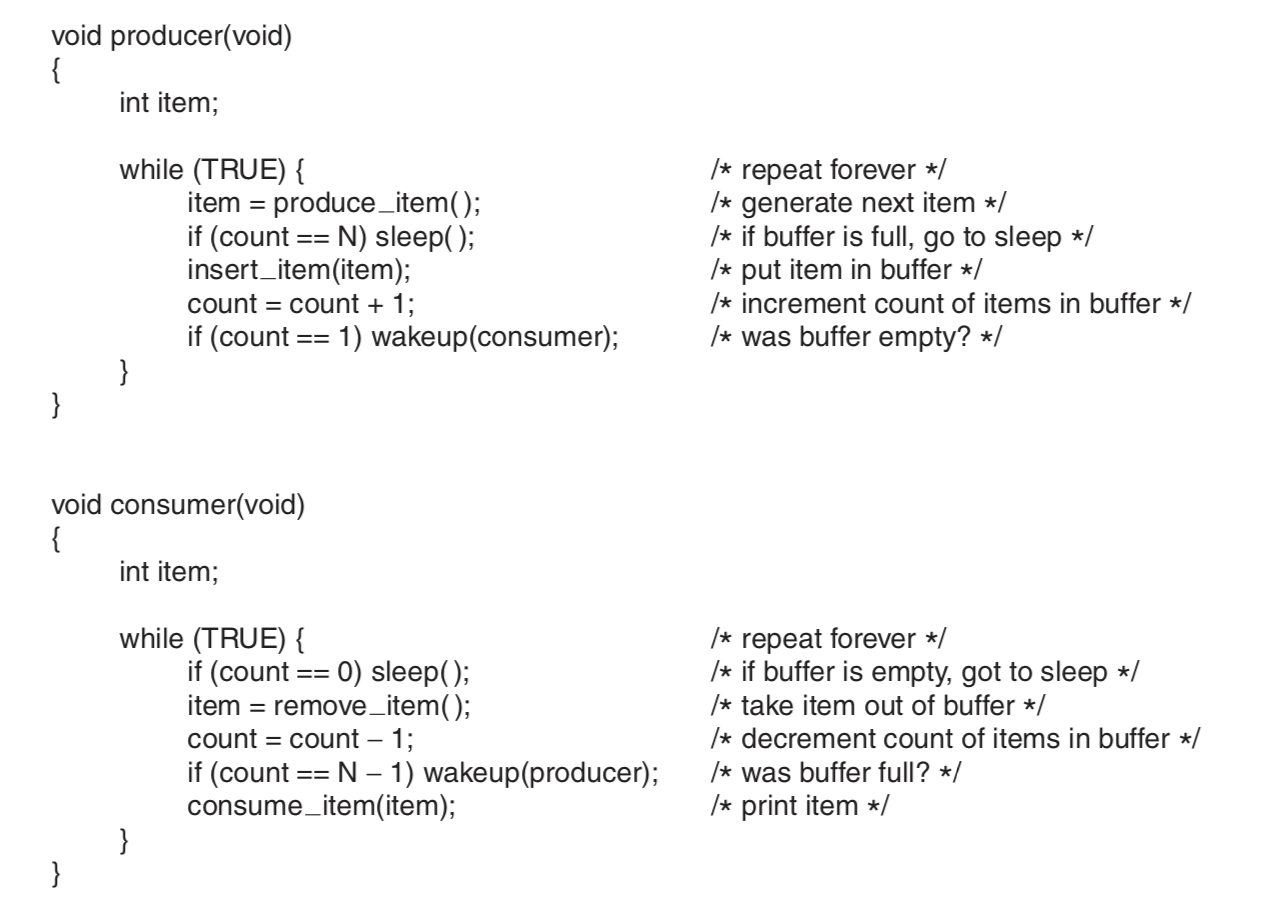
\includegraphics[width=6in]{saw.png}
\subsubsection{问题:}
\paragraph{1.}CPU执行consumer,读取到count为0。
\paragraph{2.}CPU切换至producer,producer向buffer中写入一个data,count+=1,并且producer wakeup了consumer。但由于此时consumer并没有真的sleep,这个wakeup信号失效。
\paragraph{3.}CPU切换至consumer,consumer判断count为0,进入sleep。
\paragraph{4.}CPU只能执行producer,producer最终填满了buffer,进入sleep。
\paragraph{5.}造成了死锁!
\subsubsection{问题的成因:}
\paragraph{}问题的成因就在于,我们自己实现的进程间通信,由于一些关键操作上并不是原子执行,比如consumer在读取conunt,判断count和sleep这应该是一个不可分的原子操作,才不会出现问题。
\paragraph{}在之前的忙等待实现中,也可能出现这种问题,造成死锁。
\paragraph{}因此,实现进程间的通信,一定要使用库函数。库函数能够保证一些关键操作上是原子执行,不会出现问题。

\subsection{信号量}
\subsubsection{信号量的介绍}
\paragraph{}信号量是一个用来计数的非负整数,他有两个操作,down操作和up操作,并且在初始化一个信号量的时候能够赋予一个非负初值。
\paragraph{}up操作会使信号量+=1。
\paragraph{}down操作会首先检查信号量是否为0,如果为0,会挂起当前线程;如果不为0,则会使信号量-=1。
\paragraph{}down操作保证了检查数值、修改变量值以及可能发生的sleep都是不可分割的院子操作。
\paragraph{}此外,一旦一个进程在访问一个信号量,会保证其他进程无法访问这个信号量(通过屏蔽了当前CPU的中断(不切换进程),并且通过TSL/XCHG汇编指令锁死了访问这个信号量的内存总线)。
\paragraph{}以上两个操作保证了,如果我们的信号量使用得当,不会出现像之前那种由于进程调度造成的诡异的死锁。
\paragraph{}当信号量经过up操作,其值由0变为1之后,操作系统会唤醒一个挂起在这个信号量上的线程,如果有多个,也只唤醒一个。当被唤醒的线程成功的down了之后,信号量再次变为0。
\subsubsection{用信号量解producer-consumer}
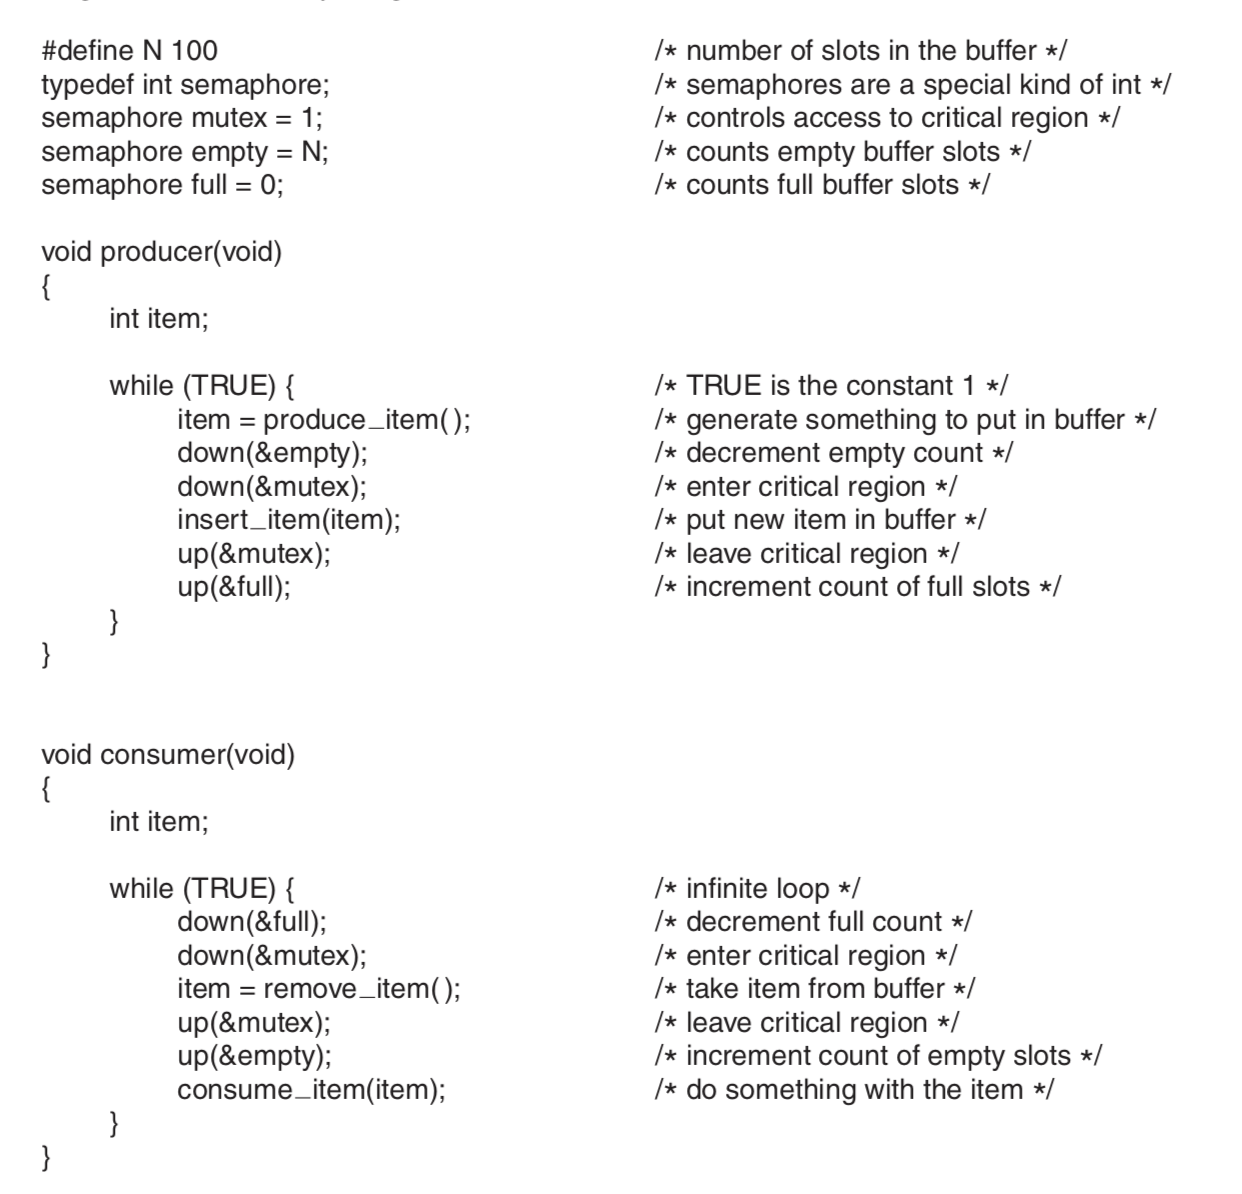
\includegraphics[width=6in]{sig.png}
\subsubsection{问题}
\paragraph{}需要注意的是,并不是说使用了信号量就不会出现死锁,信号量只是保证了在逻辑合理的情况下不出现死锁。
\paragraph{}在上述代码中,如果我们把先down(\&mutex)后down(\&empty)。考虑这种情况,buffer中已经满了,现在CPU在执行producer,producer先down了一次mutex,并且成功拿到了锁,之后再down empty,发现已经满了,empty为0,producer被挂起。CPU执行consumer,尝试down mutex,但此时mutex已经为0,down失败,consumer被挂起。发生了死锁。

\subsection{互斥量和条件变量}
\subsection{互斥量的介绍}
\paragraph{}互斥量又称互斥锁,可以认为是只有0和1两个值的信号量。
\paragraph{}两个基本操作,lock和unlock。
\paragraph{}在lock时,会先判断mutex的值是否为0,如果为0则挂起当前线程,如果为1则将mutex的值修改为1。
\paragraph{}unlock,在使用正确的情况下,只有拿到mutex的线程才会执行unlock,unlock操作后,mutex的值会变为1。
\paragraph{}pthread库中,有一个trylock方法,该方法会先判断mutex的值是否为0,如果不为0,则将mutex的值设置为0并继续执行;如果为0,则返回一个错位代码,而不是阻塞线程,给了调用者一定的灵活性。
\subsection{条件变量的介绍}
\paragraph{}有两个基本的方法,cond\_wait和cond\_signal。
\paragraph{}如果对一个线程执行了一个条件变量cond的cond\_wait的方法,那么这个线程会挂起,直到出现信号把他唤醒。
\paragraph{}如果对一个线程执行了同一个条件变量的cond\_signal,那么他将唤醒一个挂起在这个条件变量上的线程。
\paragraph{}cond\_broadcast同时唤醒所有挂起在同一个条件变量上的线程。
\subsection{用互斥量和条件变量解producer-consumer}
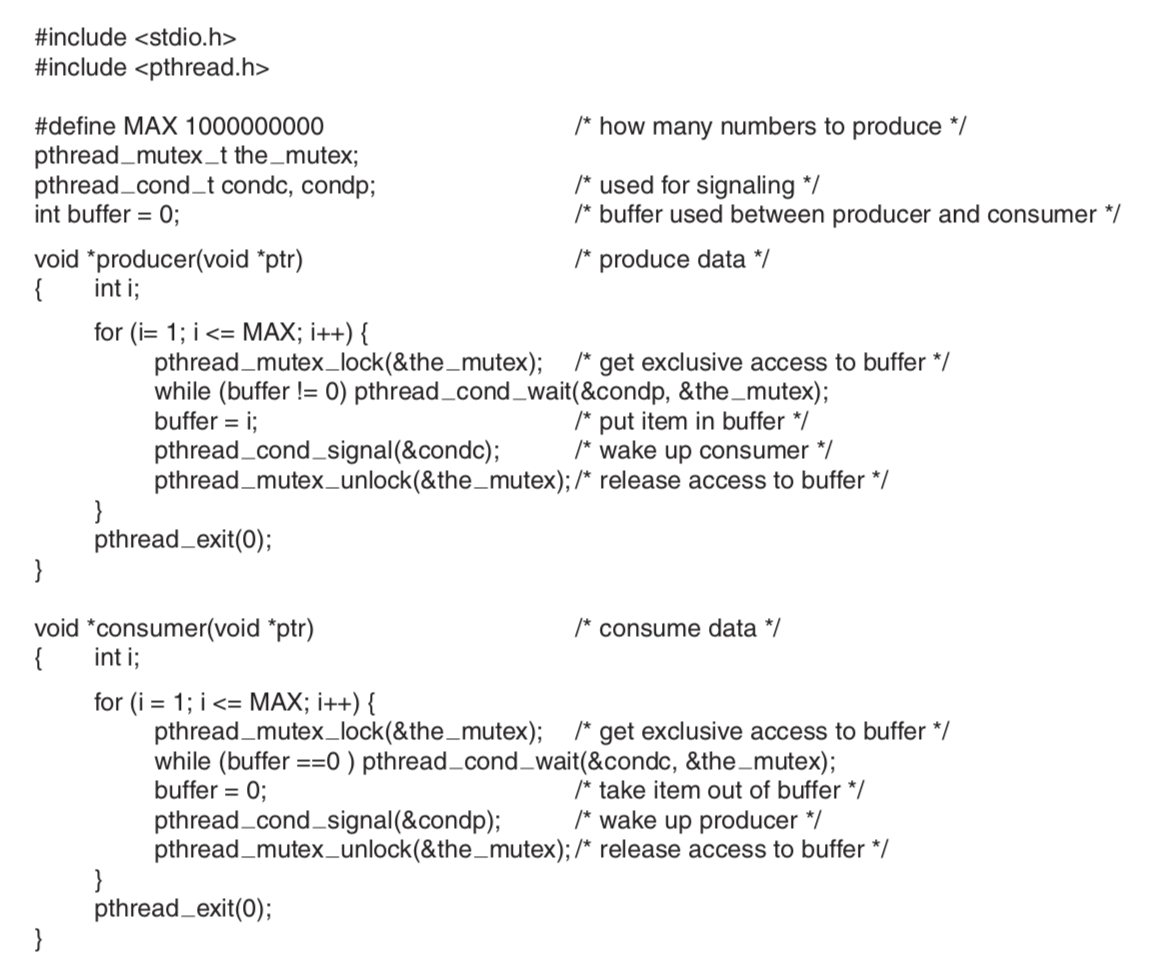
\includegraphics[width=8in]{mutex.png}

\subsection{队列}
\paragraph{}可以认为是封装好了的一个读写公共内存+有进程间通信保护的一个队列。
\subsubsection{python中的Queue}
\paragraph{1.}from multiprocessing import Queue
\paragraph{2.}q=Queue()
\\创建一个队列	
\paragraph{3.}q.put(elemets)
\\向队列中加入一个元素
\paragraph{4.}q.get(bool)
\\从队列中读取一个元素,如果队列为空的时候,如果bool为true,则会阻塞到get成功;如果bool为false,则会trow 一个error出来。







\end{CJK}
\end{document}